\section{Implementación}\label{sec:implementacion}

\begin{wrapfigure}{r}{0.5\textwidth}
    \centering
    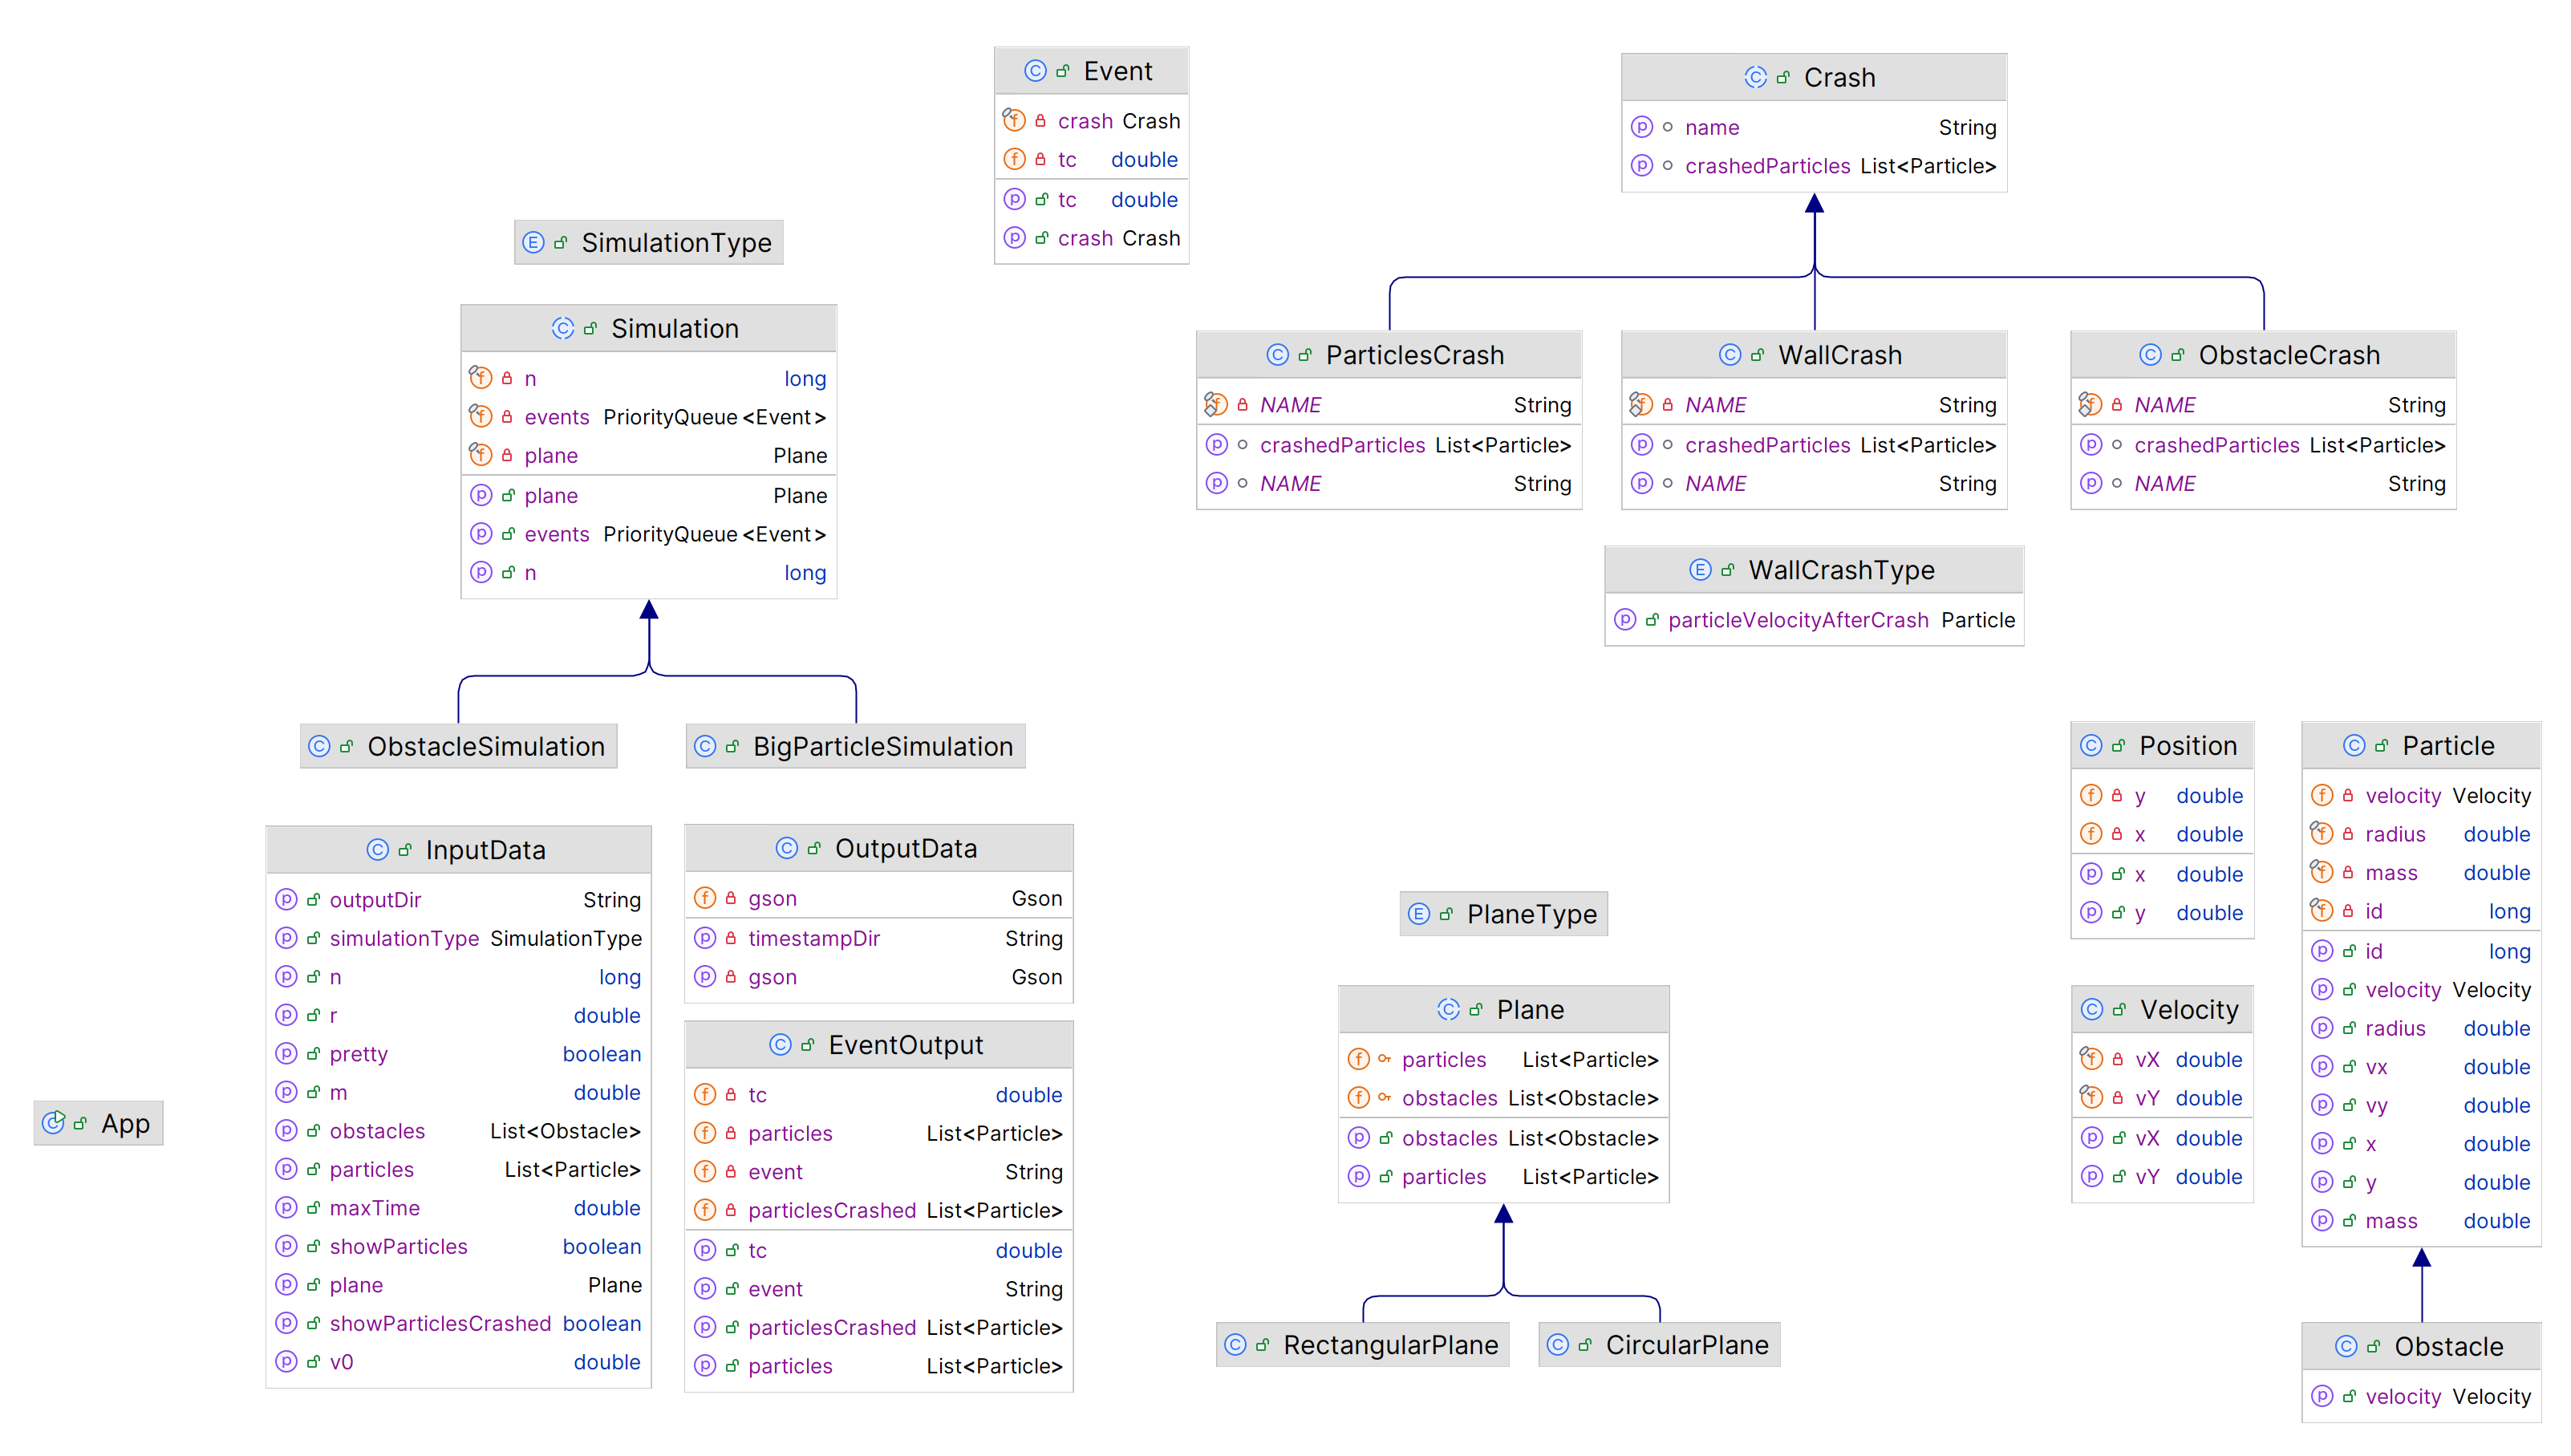
\includegraphics[width=1\linewidth]{UML}
    \caption{Diagrama UML}
    \label{fig:UML-Simulacion}
\end{wrapfigure}

\subsection{Simulación}\label{label:simulacion}
    La clase $LifeGame$ modela una instancia de la simulación del sistema. Por defecto las reglas son las del juego de la vida,
    pero es posible modificar las condiciones para poder simular sistemas alternativos. Esta clase es el nucleo de la
    simulación (Ver diagrama UML~\ref{fig:UML-Simulacion}), debido a que posee todos los componentes necesarios
    para representar una instancia particular del sistema. $LifeGameRunner$ controlara el flujo y evolucion del sistema,
    siendo invocado por $App$ que es el punto de entrada al codigo.

\subsection{Matriz de celdas}\label{subsec:matriz de celdas}
    En lo que refiere a la simulación del modelo, este ha sido diseñado para trabajar con automatas celulares de tres
    dimensiones, ya que toda posicion comprende las componentes x, y, z (Ver $Position$ en diagrama UML~\ref{fig:UML-Simulacion}).
    En caso de ser bidimensional, toda posicion tendra $z = 0$.

    En esta implementación se ha optado por una representación eficiente de la matriz de celdas utilizando una coleccion de
    tipo Set en lugar de una estructura matricial convencional.
    La presencia de una celda en el set indica que dicha celda está viva, mientras que la ausencia de la Position en
    el conjunto implica que la celda está muerta.

\subsection{Condiciones de corte}\label{label:condiciones_de_corte}
    La simulación puede finalizar por cuatro razones diferentes. Representadas como una enumeracion de JAVA, estas son:
    \begin{itemize}
        \item $BORDER$: Ocurre cuando se alcanza un paso donde existe una celda aledaña a un borde de la matriz.
        \item $ALL\_DEAD$: Ocurre en el caso de que se alcanza un paso que no tenga celdas vivas.
        \item $MAX\_ITER$: Al alcanzar una cantidad maxima de iteraciones en la simulación. Esta cantidad es parametro de
            entrada de la simulación.
        \item $NO\_CHANGE$: Cuando no hay variacion de la matriz de celdas entre dos pasos consecutivos.
    \end{itemize}

\subsection{Código auxiliar}\label{label:codigo_aux}
    Se implementan diversas clases y métodos para tareas auxiliares. En el caso de $InputData$ se provisionan métodos
    para la lectura y escritura de archivos JSON para poder parametrizar la simulación en función a un archivo de entrada.
    La salida en un archivo JSON es utilizada para registrar los resultados de la simulación.

    Adicionalmente, las clases $Border$, $Position$ y $NeighbourhoodCondition$ modelan el comportamiento de la matriz de
    celdas. En primer lugar $Border$ simplemente modela las dimensiones de la matriz de celdas de la instancia particular
    del sistema a modelar. Por otro lado $Position$ es la representación de una celda dentro de la matriz.Por ultimo,
    NeighbourhoodCondition es una enumeración de JAVA que implementa un método que retorna, para un determinado rango
    $r$, las celdas vecinas de una celda central segun el tipo de vecindario.